\chapter{Benutzerschnittstellen}

\section{Kommandozeile}\label{sec:uicmd}

Die Kommandozeilen-Schnittstelle bietet dem Benutzer eine schnelle Möglichkeit Graphdateien beim Programmstart mit zusätzlichen Parametern zu öffnen.
Folgende Parameter werden unterstützt:\\
\subsection{Muss-Argumente}
\begin{tabular}{lp{0.75\linewidth}}
  -layout <layout> & Legt einen Layout-Algorithmus fest, welcher beim Programmstart auf den ersten Graphen angewendet wird.\\
    & Dabei ist <layout> ein Kürzel, das vom jeweiligen Layout-Plugin definiert wird. Das Kürzel wird hinter der Layout-Option in der Menüleiste angezeigt.\\
  -in <datei> & Legt die zu öffnende Graphdatei fest. <datei> ist der relative oder absolute Pfad zu einer Graphdatei. Alternativ kann ``-in'' weggelassen werden, falls der Pfad als letztes Argument angegeben wird.\\
  -type <typeid> & Legt den Typ des Graphen fest. Über den Typ des Graphen wird das Import-Plugin, sowie initiale Darstellungsoptionen festgelegt. Graphtypen können von Plugins definiert werden. (siehe ) %TODO: Referenz Pluginsschnittstellen)
\end{tabular}

\subsection{Kann-Argumente}
\begin{tabular}{lp{0.75\linewidth}}
  -out <datei> & Legt einen Pfad zu einer Datei fest, in welcher der Graph gespeichert werden soll.
  Es wird die in %TODO: Referenz zu Kann Funktion zum speichern von graphen
  beschrieben Funktion ausgeführt.
  Falls angegeben, wird der Layout-Algorithmus auf alle Graphen in der zu öffnenden Datei angewendet, bevor das Speichern beginnt.
  Die \gls{gui} wird nicht gestartet.
\end{tabular}

\section{GUI}\label{sec:uigui}

Die graphische Oberfläche bietet dem Benutzer ein interaktives Interface und eine Anzeige für die gelayouteten Graphen. %TODO: gelayoutet ersetzen

\subsection{Entwürfe}

\begin{figure}[ht]
  \centering
  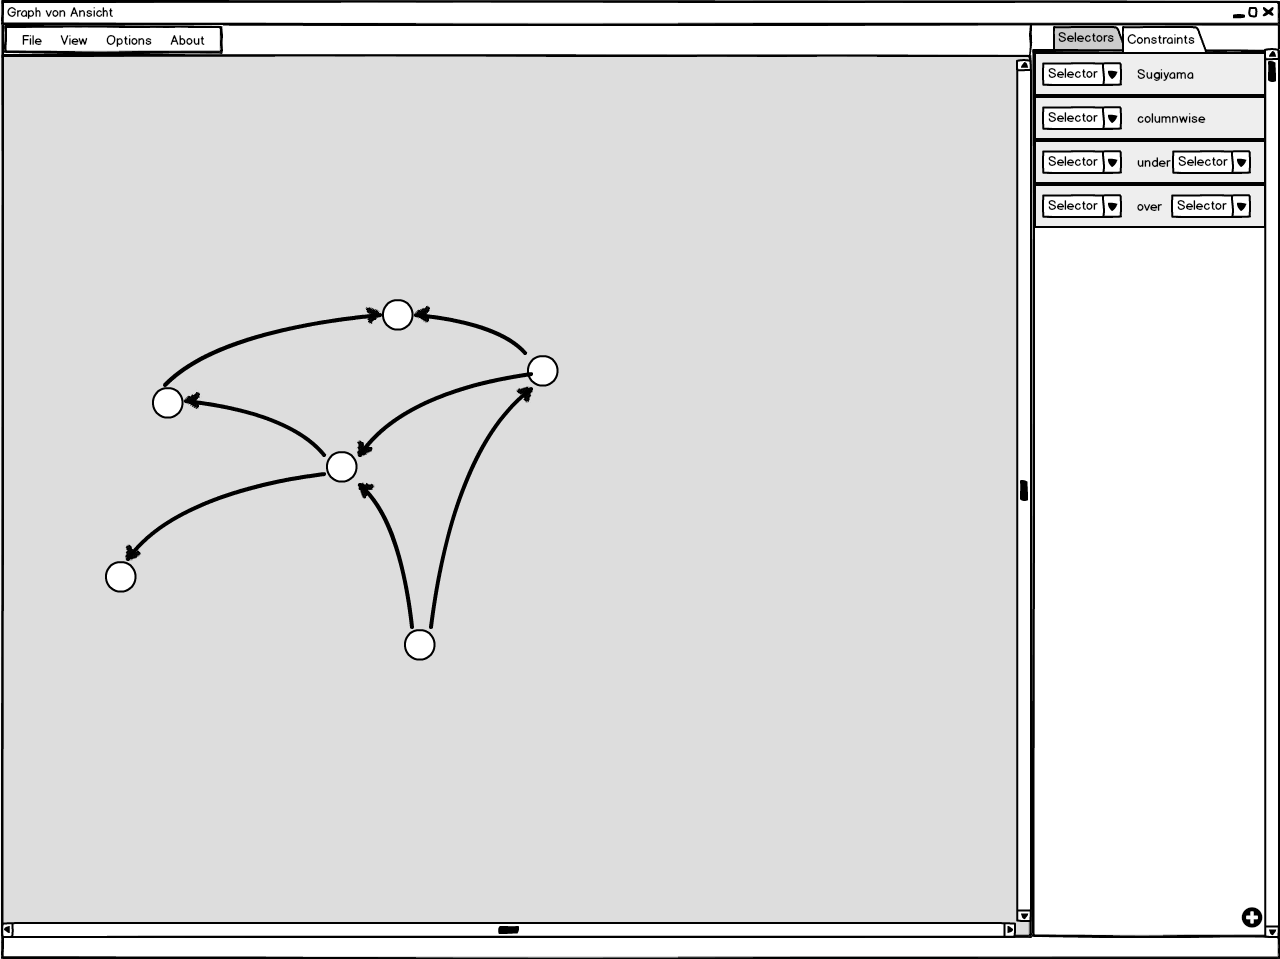
\includegraphics[width=300pt]{resourcen/main.png}
  \caption{Hauptansicht}
  \label{fig:mainView}
\end{figure}

\begin{figure}[ht]
  \centering
  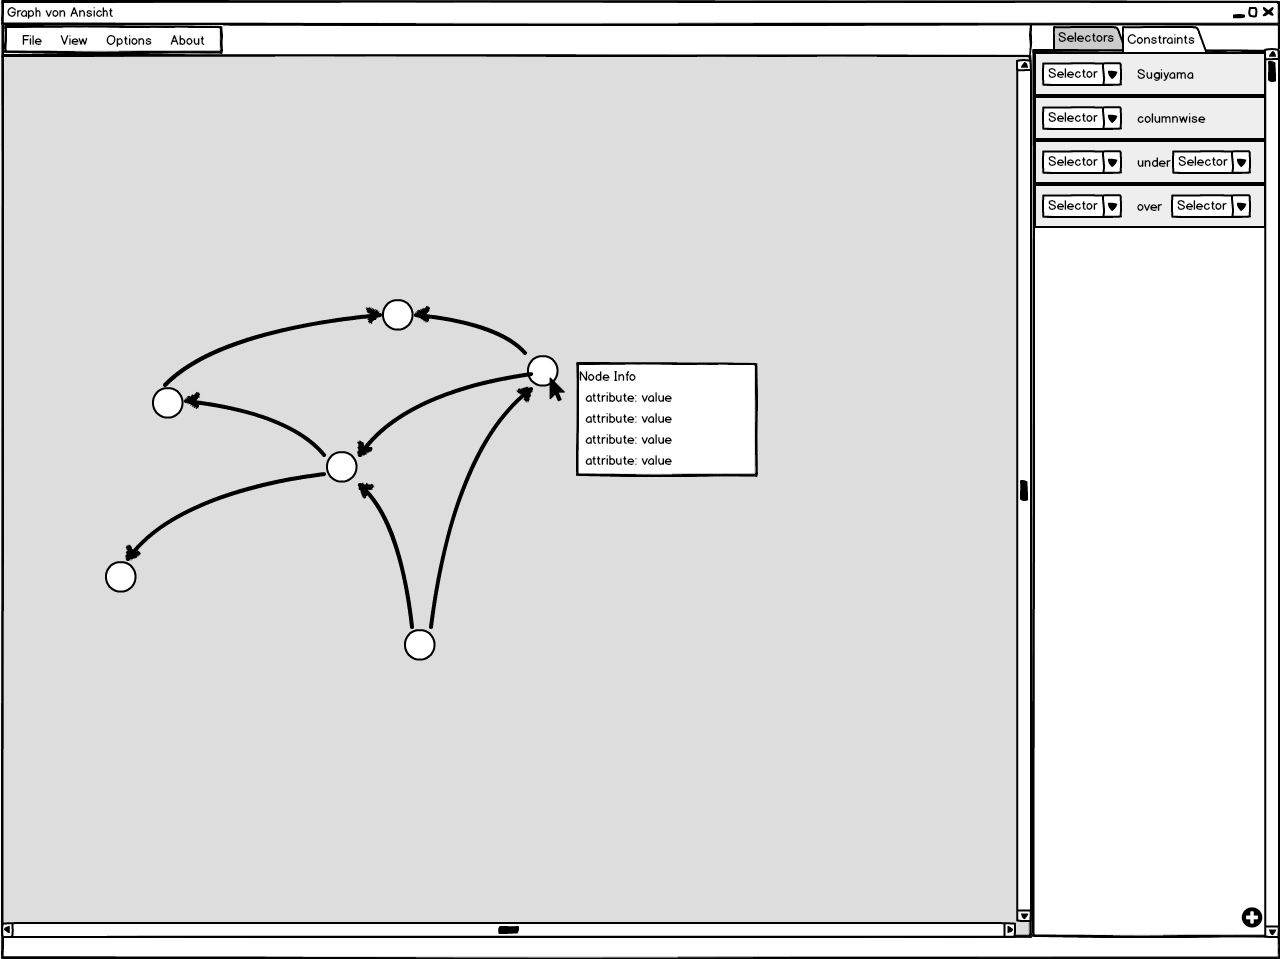
\includegraphics[width=300pt]{resourcen/nodeInfo.png}
  \caption{Knoteninformation}
  \label{fig:nodeInfo}
\end{figure}

\begin{figure}[ht]
  \centering
  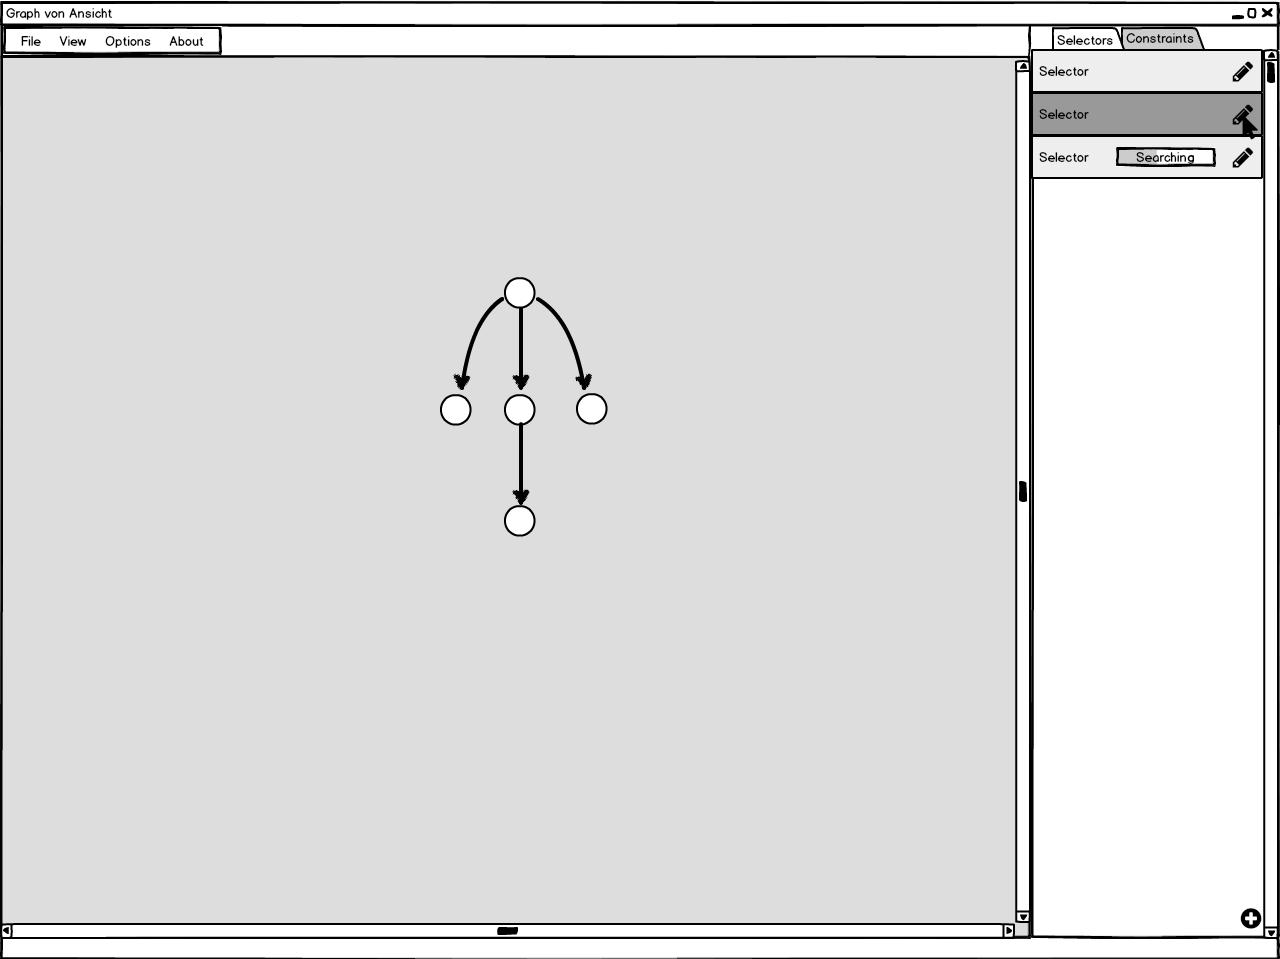
\includegraphics[width=300pt]{resourcen/selectSelector.png}
  \caption{Selektoren Ansicht}
  \label{fig:selectorView}
\end{figure}